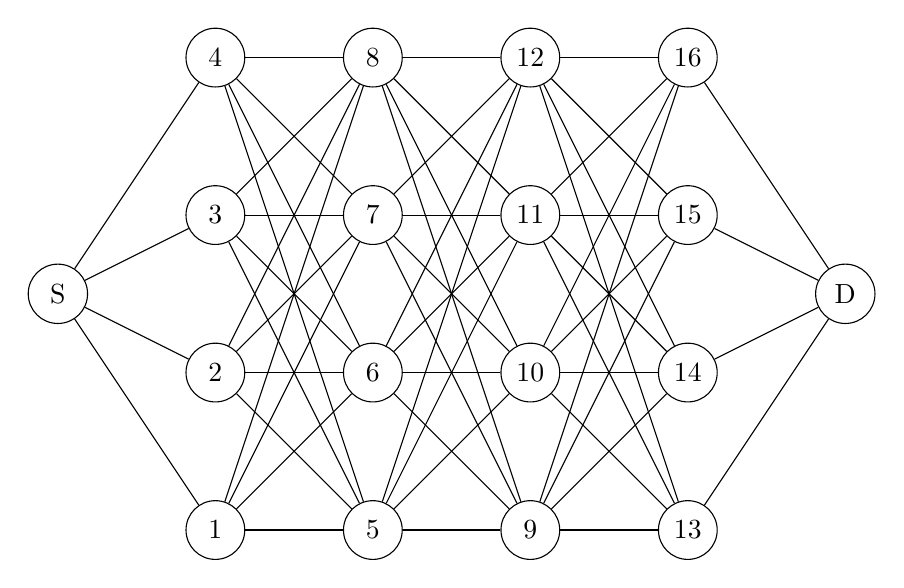
\begin{tikzpicture}

\def \n {4}
\def \radius {3cm}

\tikzset{vertex/.style = {align=center, text centered, draw, circle, text width=1em}}

\node[vertex] (S) at (2, 5) {S};
\node[vertex] (D) at ({2 * (2 + \n)}, 5) {D};

\foreach \i in {1,...,\n}
{
	\foreach \j in {1,...,\n}
	{
		\pgfmathtruncatemacro{\num}{(\i - 1) * \n + \j}
		\node[vertex] (\num) at ({2 * (\i + 1)}, {2 * \j}) {\num};
	}
}

\foreach \i in {1,...,\n}
{
	\pgfmathtruncatemacro{\vi}{\i}
	\draw[-] (\vi) edge (S);
}

\foreach \i in {1,...,\n}
{
	\pgfmathtruncatemacro{\vi}{(\n - 1) * \n + \i}
	\draw[-] (\vi) edge (D);
}

\foreach \i in {2,...,\n}
{
	\foreach \j in {1,...,\n}
	{
		\foreach \k in {1,...,\n}
		{
			\pgfmathtruncatemacro{\vi}{(\i - 2) * \n + \j}
			\pgfmathtruncatemacro{\vj}{(\i - 1) * \n + \k}
			\draw[-] (\vi) edge (\vj);
		}
	}
}

\end{tikzpicture}
